\section{Technischer Hintergrund}
\subsection{ Beschleunigungssensoren}
\noindent In diesem Versuch wurden zu einem ein IPhone 12 mini und ein IPhone 11 verwendet. 
Für die Messung wurde ein \textit{iPhone 12 mini} (Modell: iPhone13,1) verwendet. Das Gerät stammt vom Hersteller Apple, die verwendete Stichprobengröße basiert auf 292 Geräten, wobei es sich um eine Gerätevariante handelt. Das integrierte \textbf{Beschleunigungssensor-Modul (Accelerometer)} des iPhones ist verfügbar und weist folgende Eigenschaften auf \cite{phyphoxSensorDB}:
\begin{itemize}
  \item \textbf{Abtastrate:} 100{,}0\,Hz
  \item \textbf{Durchschnittlicher Beschleunigungswert (im Ruhezustand):} 9{,}820\,m/s\textsuperscript{2}
  \item \textbf{Standardabweichung:} 0{,}018\,m/s\textsuperscript{2}
\end{itemize}
\noindent Diese Werte deuten auf eine hohe Genauigkeit und Stabilität des Sensors hin, was ihn für Bewegungsanalysen – wie beispielsweise die Bestimmung des Kniewinkels bei Kniebeugen – geeignet macht.
\\
\\
Zusätzlich kam ein \textit{iPhone 11} (Modell: iPhone12,1) zum Einsatz. Auch dieses Gerät stammt vom Hersteller Apple. Die zugrunde liegende Stichprobengröße umfasst 696 Geräte, wobei ebenfalls nur eine Gerätevariante berücksichtigt wurde. Der integrierte \textbf{Beschleunigungssensor (Accelerometer)} des iPhone 11 besitzt folgende Eigenschaften \cite{phyphoxSensorDB}:
\begin{itemize}
  \item \textbf{Abtastrate:} 100{,}0\,Hz
  \item \textbf{Durchschnittlicher Beschleunigungswert (im Ruhezustand):} 9{,}840\,m/s\textsuperscript{2}
  \item \textbf{Standardabweichung:} 0{,}015\,m/s\textsuperscript{2}
\end{itemize} 
\noindent Diese technischen Daten belegen ebenfalls eine hohe Genauigkeit und geringe Streuung der Sensordaten, was die Eignung des Geräts für präzise Bewegungsanalysen wie Kniebeugenmessungen bestätigt. 

\subsection{Phyphox-App}
Damit die Bewertung einer Kniebeuge von jeder Person durchgeführt werden kann, wird die kostenlose App \textit{Phyphox} verwendet. \textit{Phyphox} ist eine Marke der RWTH Aachen, eingetragen in Deutschland, der EU, den USA und anderen Ländern. \noindent Die App \textit{Phyphox} kann kostenlos auf Smartphones installiert werden \cite{phyphoxDownload}. 
Für iOS-Geräte ist sie im \href{https://apps.apple.com/us/app/phyphox/id1127319693?l=de&ls=1}{App Store} erhältlich, 
für Android-Geräte im \href{https://play.google.com/store/apps/details?id=de.rwth_aachen.phyphox}{Google Play Store}.
\\
\noindent Die App umfasst verschiedene Funktionen, zu einem können die Sensoren des Smartphones verwendet werden um zu experimentieren, es ist ein Daten Export in verschiedenen Formaten möglich, es ist eine Fernsteuerung zu einem Web-Browser möglich, und es können eigene Experimente erstellt werden. In der App stehen einem viele Möglichkeiten zur Verfügung. Es wird unterschieden in Sensoren, Akustik, Alltag, Mechanik, Werkzeuge und Zeitmessung. In der Abbildung 4 sind die einzelnen Auswahlmöglichkeiten der Kategorien ersichtlich. \cite{Phyphox}
\begin{figure}[ht]\centering
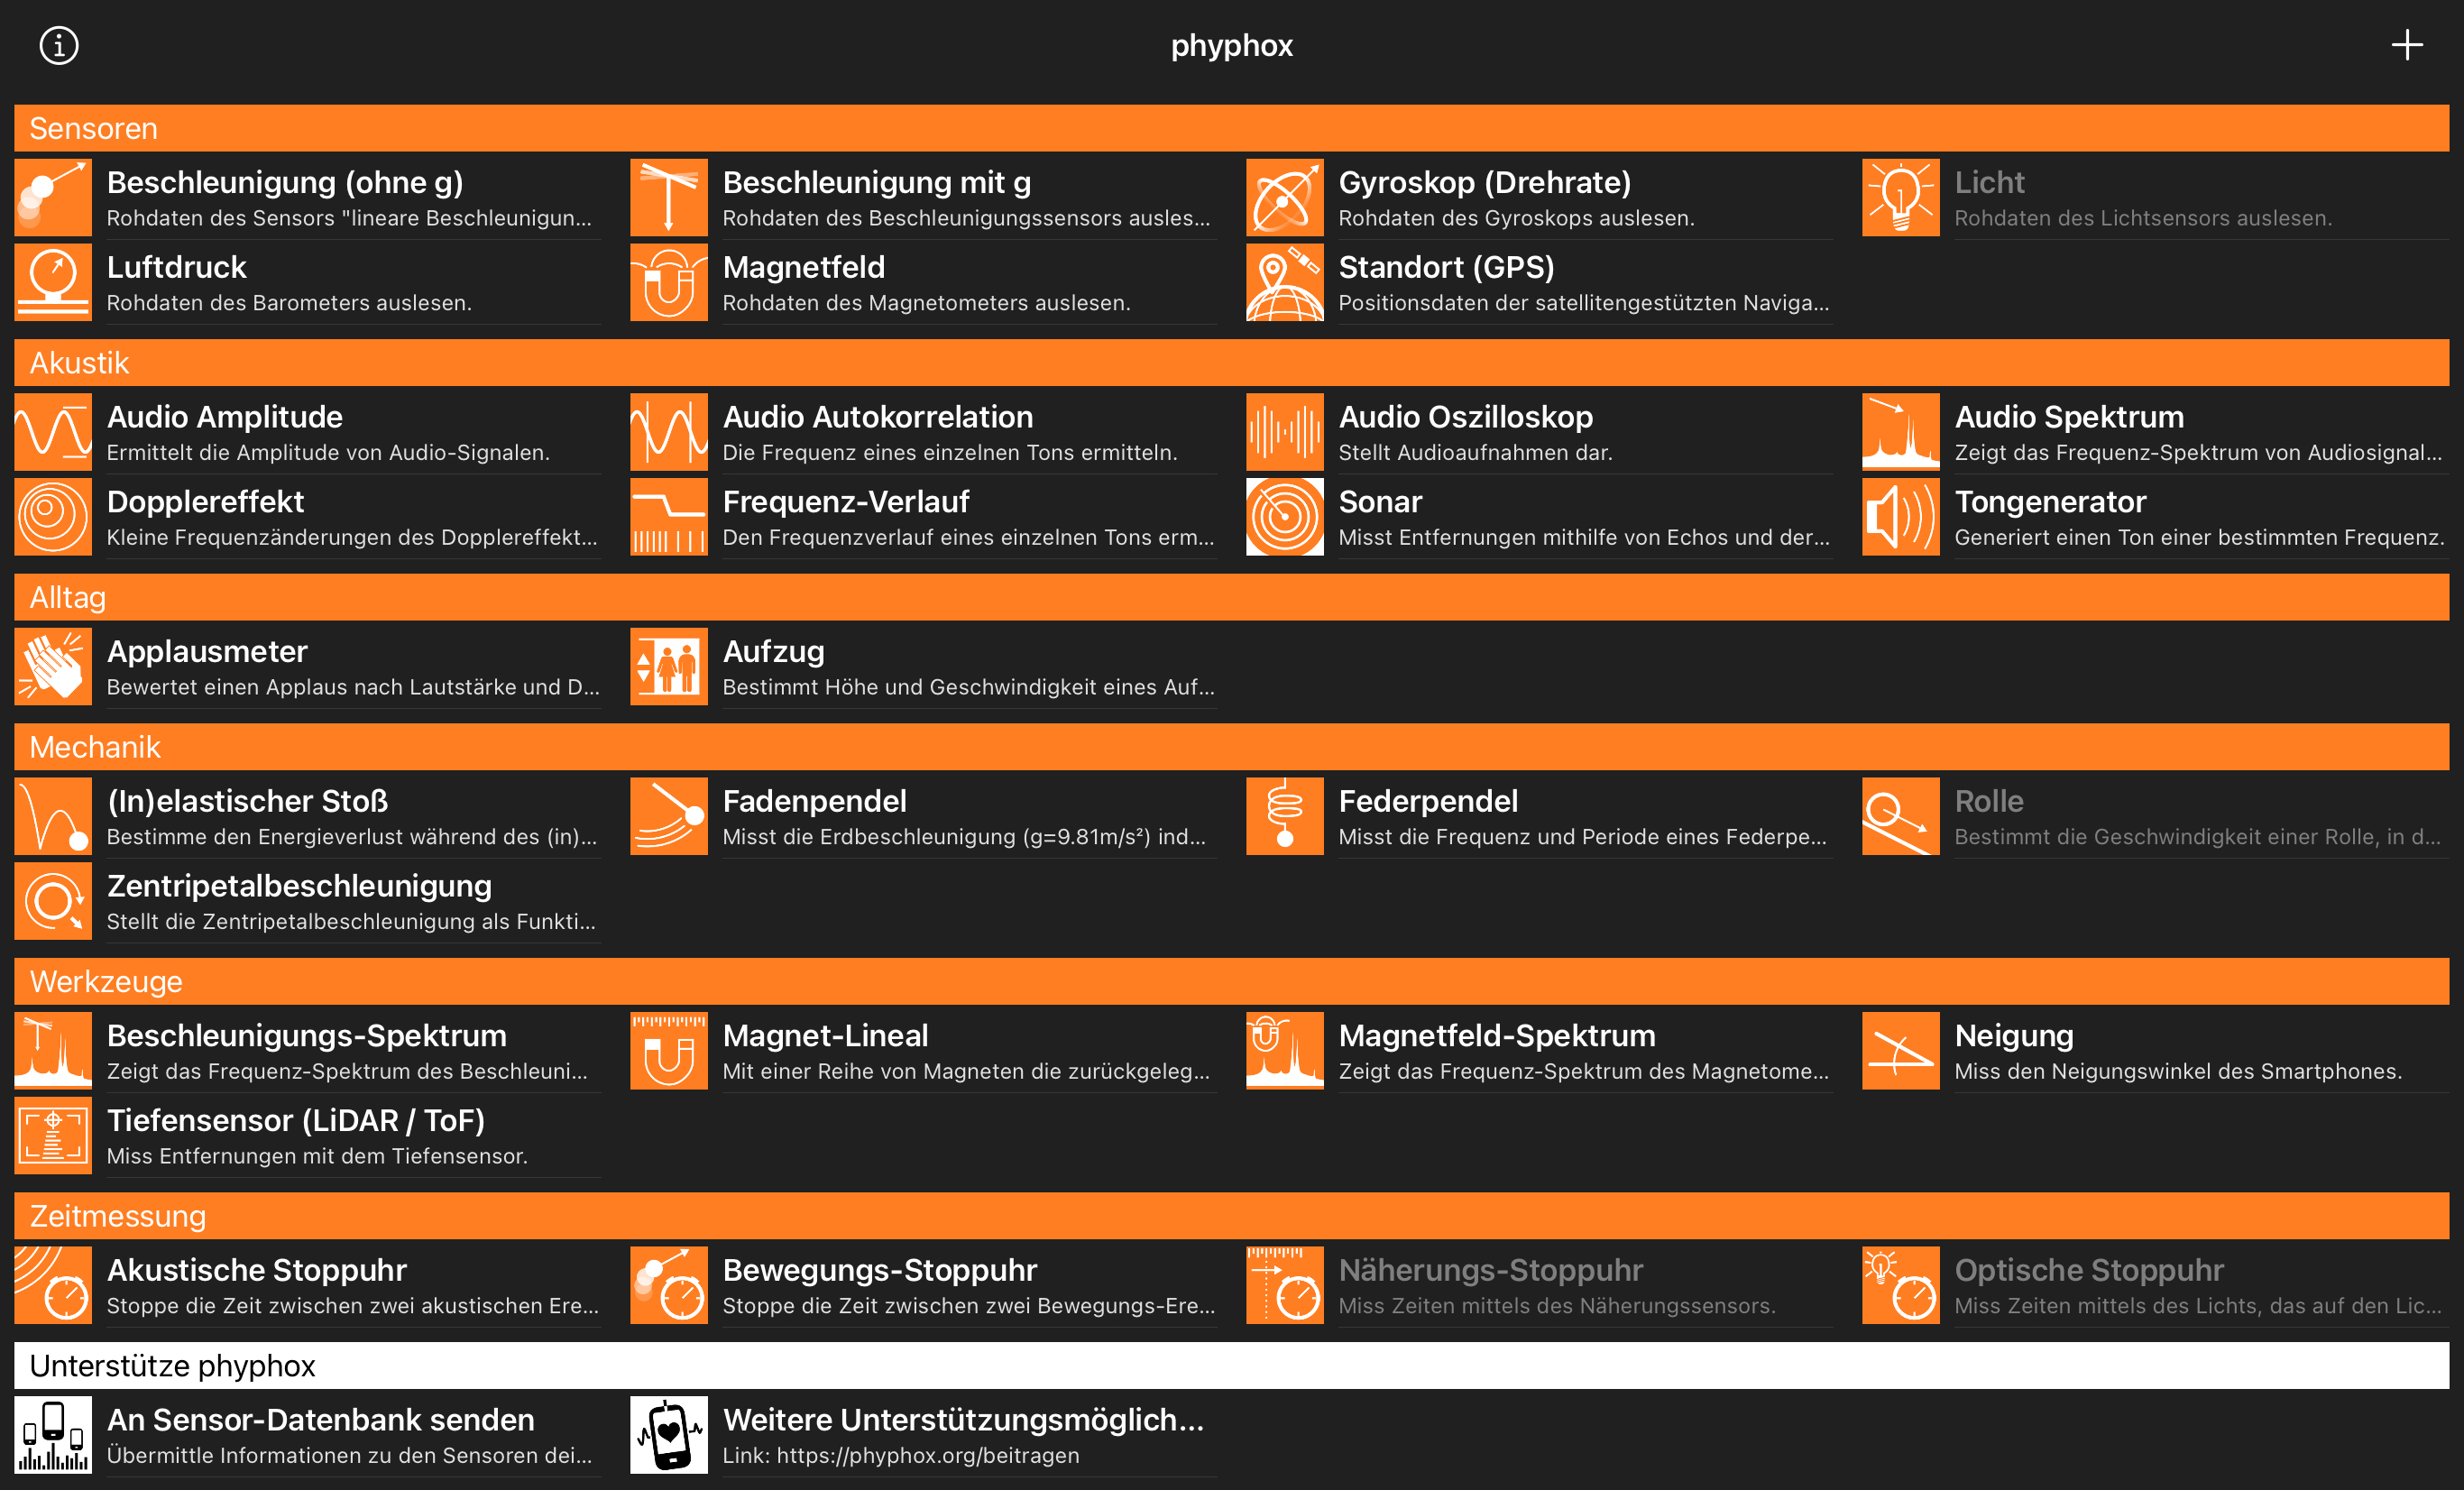
\includegraphics[width=\linewidth]{images/Phyphox.jpeg}
\caption{Anwenderoberfläche Phyphox \cite{Phyphox}}
\label{fig:Anwenderoberfläche Phyphox}
\end{figure}

\noindent Für die Aufnahme der Beschleunigungsdaten, die zur Auswertung der Kniebeuge benötigt werden, wird in der Kategorie Sensoren der Tab Beschleunigung mit G ausgewählt. Dadurch können die Daten des im Smartphone integrierten Beschleunigungssensors erfasst werden. Dabei wird die Gravitationskraft berücksichtigt, sodass konstant eine Beschleunigung auch ohne Bewegung von 9,81 m/s² angezeigt wird. \cite{Phyphox} Jenachdem in welcher Lage sich das Smartphone befindet, werden die Beschleunigung unterschiedlich auf die Achsen verteilt.
\\
\noindent Die Abbildung 5 veranschaulicht den Ablauf der Datenerhebung und des Exports mit der Smartphone-Applikation \textit{Phyphox} am Beispiel des Sensors „Beschleunigung mit g“. Nach dem Öffnen der App wird zunächst das entsprechende Sensor-Modul ausgewählt, das die dreidimensionale Beschleunigung unter Berücksichtigung der Gravitationskomponente erfasst (erstes Bild von links). Mit Betätigung der Aufnahmetaste wird die Messung gestartet (zweites Bild), wobei die Beschleunigungswerte in den Raumrichtungen x, y und z über die Zeit hinweg aufgezeichnet und grafisch dargestellt werden. Nach Beendigung der Aufnahme (drittes Bild) kann das Aktionsmenü (Symbol mit drei Punkten) geöffnet werden (viertes Bild). Über die Option „Daten exportieren“ (fünftes Bild) öffnet sich das Dialogfenster (sechses Bild) um das gewünschte Dateiformat für den Export auszuwählen. Für die Weiterverarbeitung der Messdaten in Programmen wie MATLAB oder Excel empfiehlt sich die Auswahl des CSV-Formats mit Komma als Dezimaltrennzeichen (CSV (Comma, decimal point)). Der Export der aufgezeichneten Daten erfolgt anschließend durch Auswahl des Buttons „Daten exportieren“.
\begin{figure}[ht]\centering
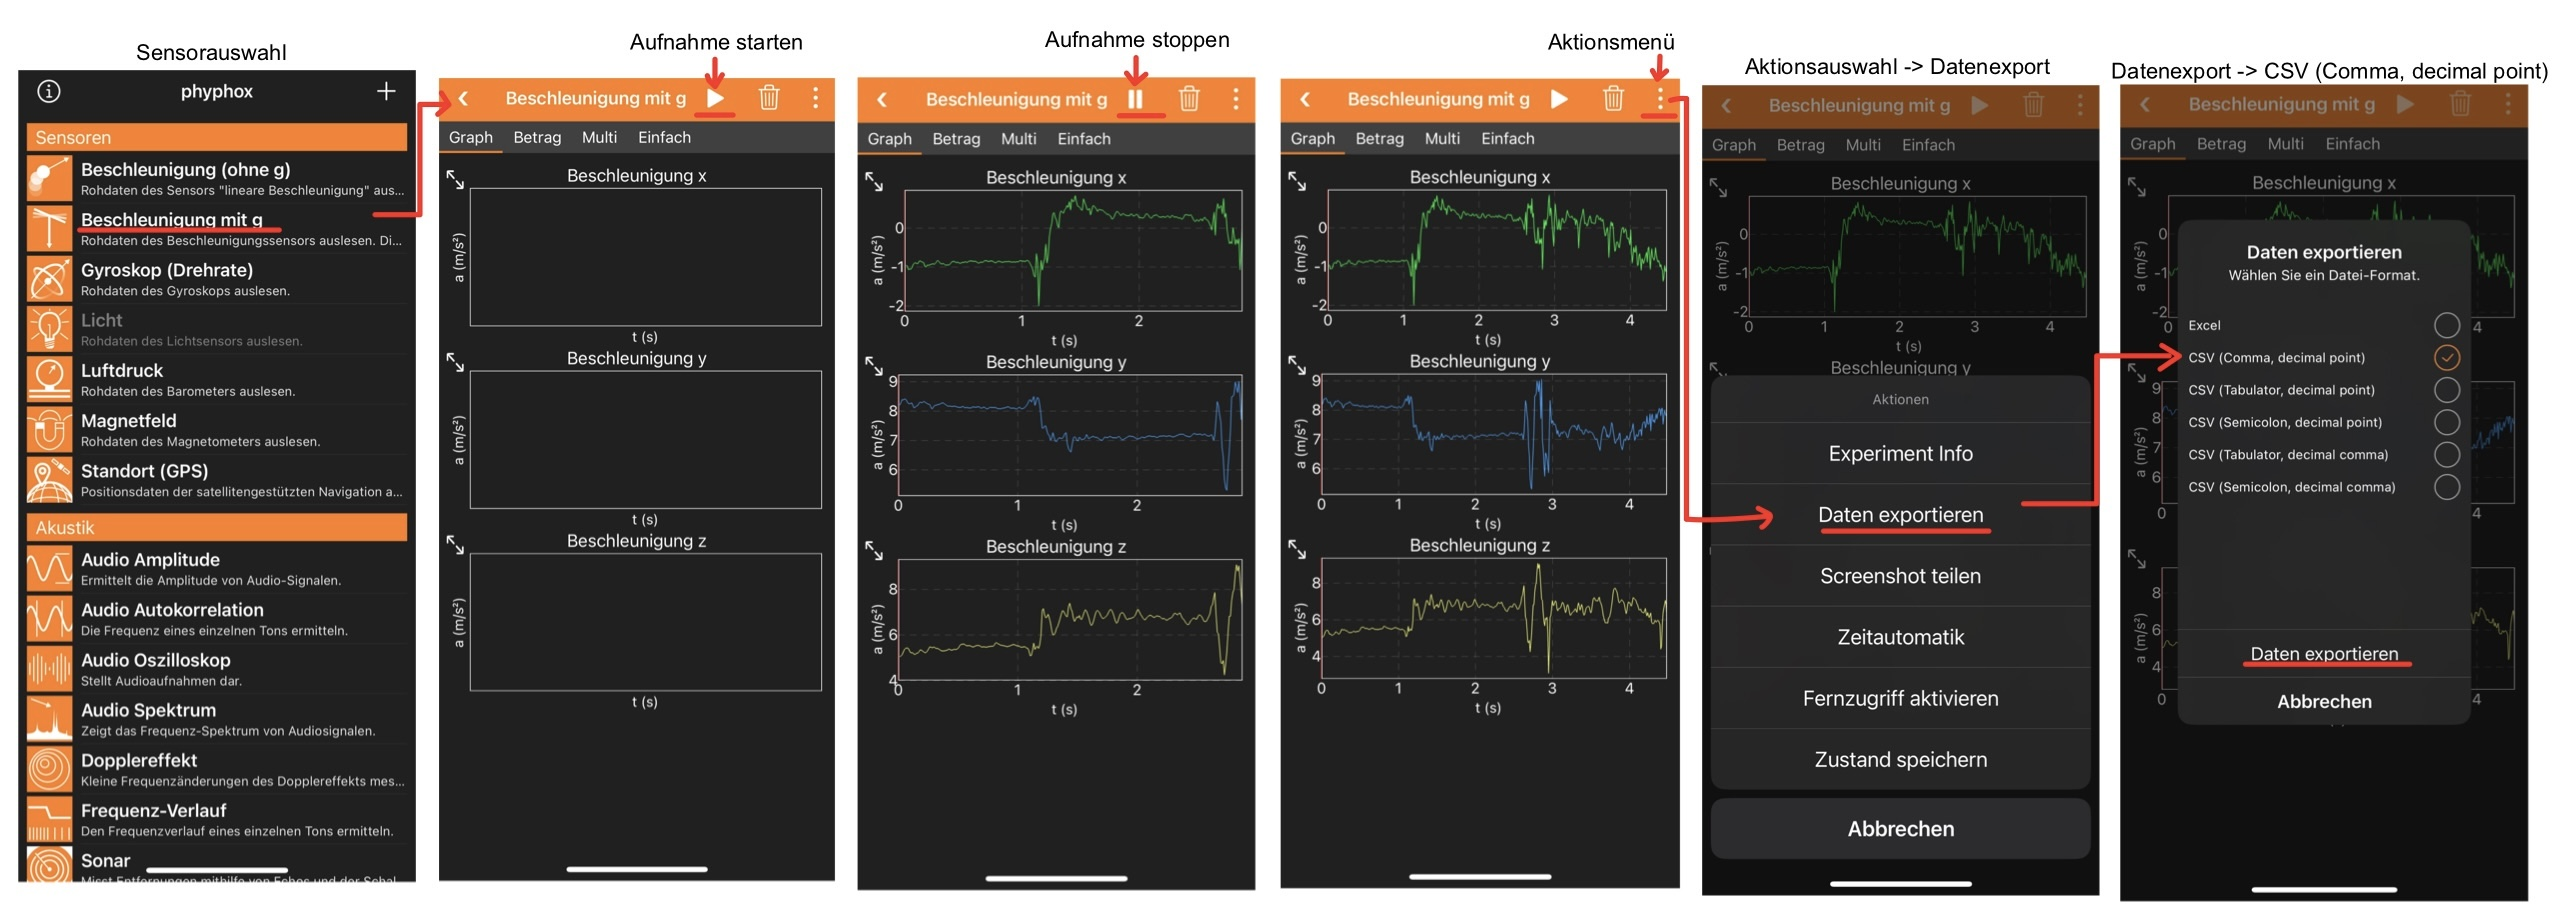
\includegraphics[width=\linewidth]{images/Bedienung.jpeg}
\caption{Bedienung Phyphox am Beispiel Beschleunigung mit g\cite{Phyphox}}
\label{fig:Anwenderoberfläche Phyphox}
\end{figure}
\subsection{Experiment zur Darstellung der App}
\noindent Im folgenden wird ein kleines Experiment untersucht, welches die Messung der Erdbeschleunigung mit einem Smartphone darstellt. Aus der Kategorie Sensoren wird der Tab Beschleunigung mit g ausgewählt. Nach dem Start über den Play-Button oben rechts, befindet sich das Smartphone zunächst flach auf dem Tisch. Danach wird es auf die Längskante gekippt und schließlich hochkant aufgestellt. Während des gesamten Versuchs erfasst der Sensor die Beschleunigung in den verschiedenen Positionen.
\\
\noindent In der Abbildung 6 sind die Messdaten des Experiments dargestellt. Die grüne Kurve zeigt die Beschleunigung entlang der X-Achse, die blaue Kurve die Beschleunigung entlang der Y-Achse, die gelbe Kurve die Beschleunigung entlang der Z-Achse und die weiße Kurve die absolute Beschleunigung. Die Werte unter dem Graphen geben die gemessene Beschleunigung zum Zeitpunkt des Stopps des Experiments an. In diesem Fall wurde die Option “Multi” ausgewählt, wodurch alle Kurven in einem gemeinsamen Diagramm dargestellt werden. Alternativ besteht die Möglichkeit, die einzelnen Achsen in separaten Diagrammen darzustellen. Diese Funktion steht unter der Option “Graph” zur Verfügung. 
\noindent Um die Achsenzuordnung genauer nachvollziehen zu können, ist diese in Abbildung 7 dargestellt. Die Abbildung 7 zeigt die Orientierung der X-, Y- und Z-Achse relativ zum Smartphone, wie sie in der verwendeten App zur Beschleunigungsmessung Phyphox verwendet wird.
\\
\begin{figure}[ht]\centering
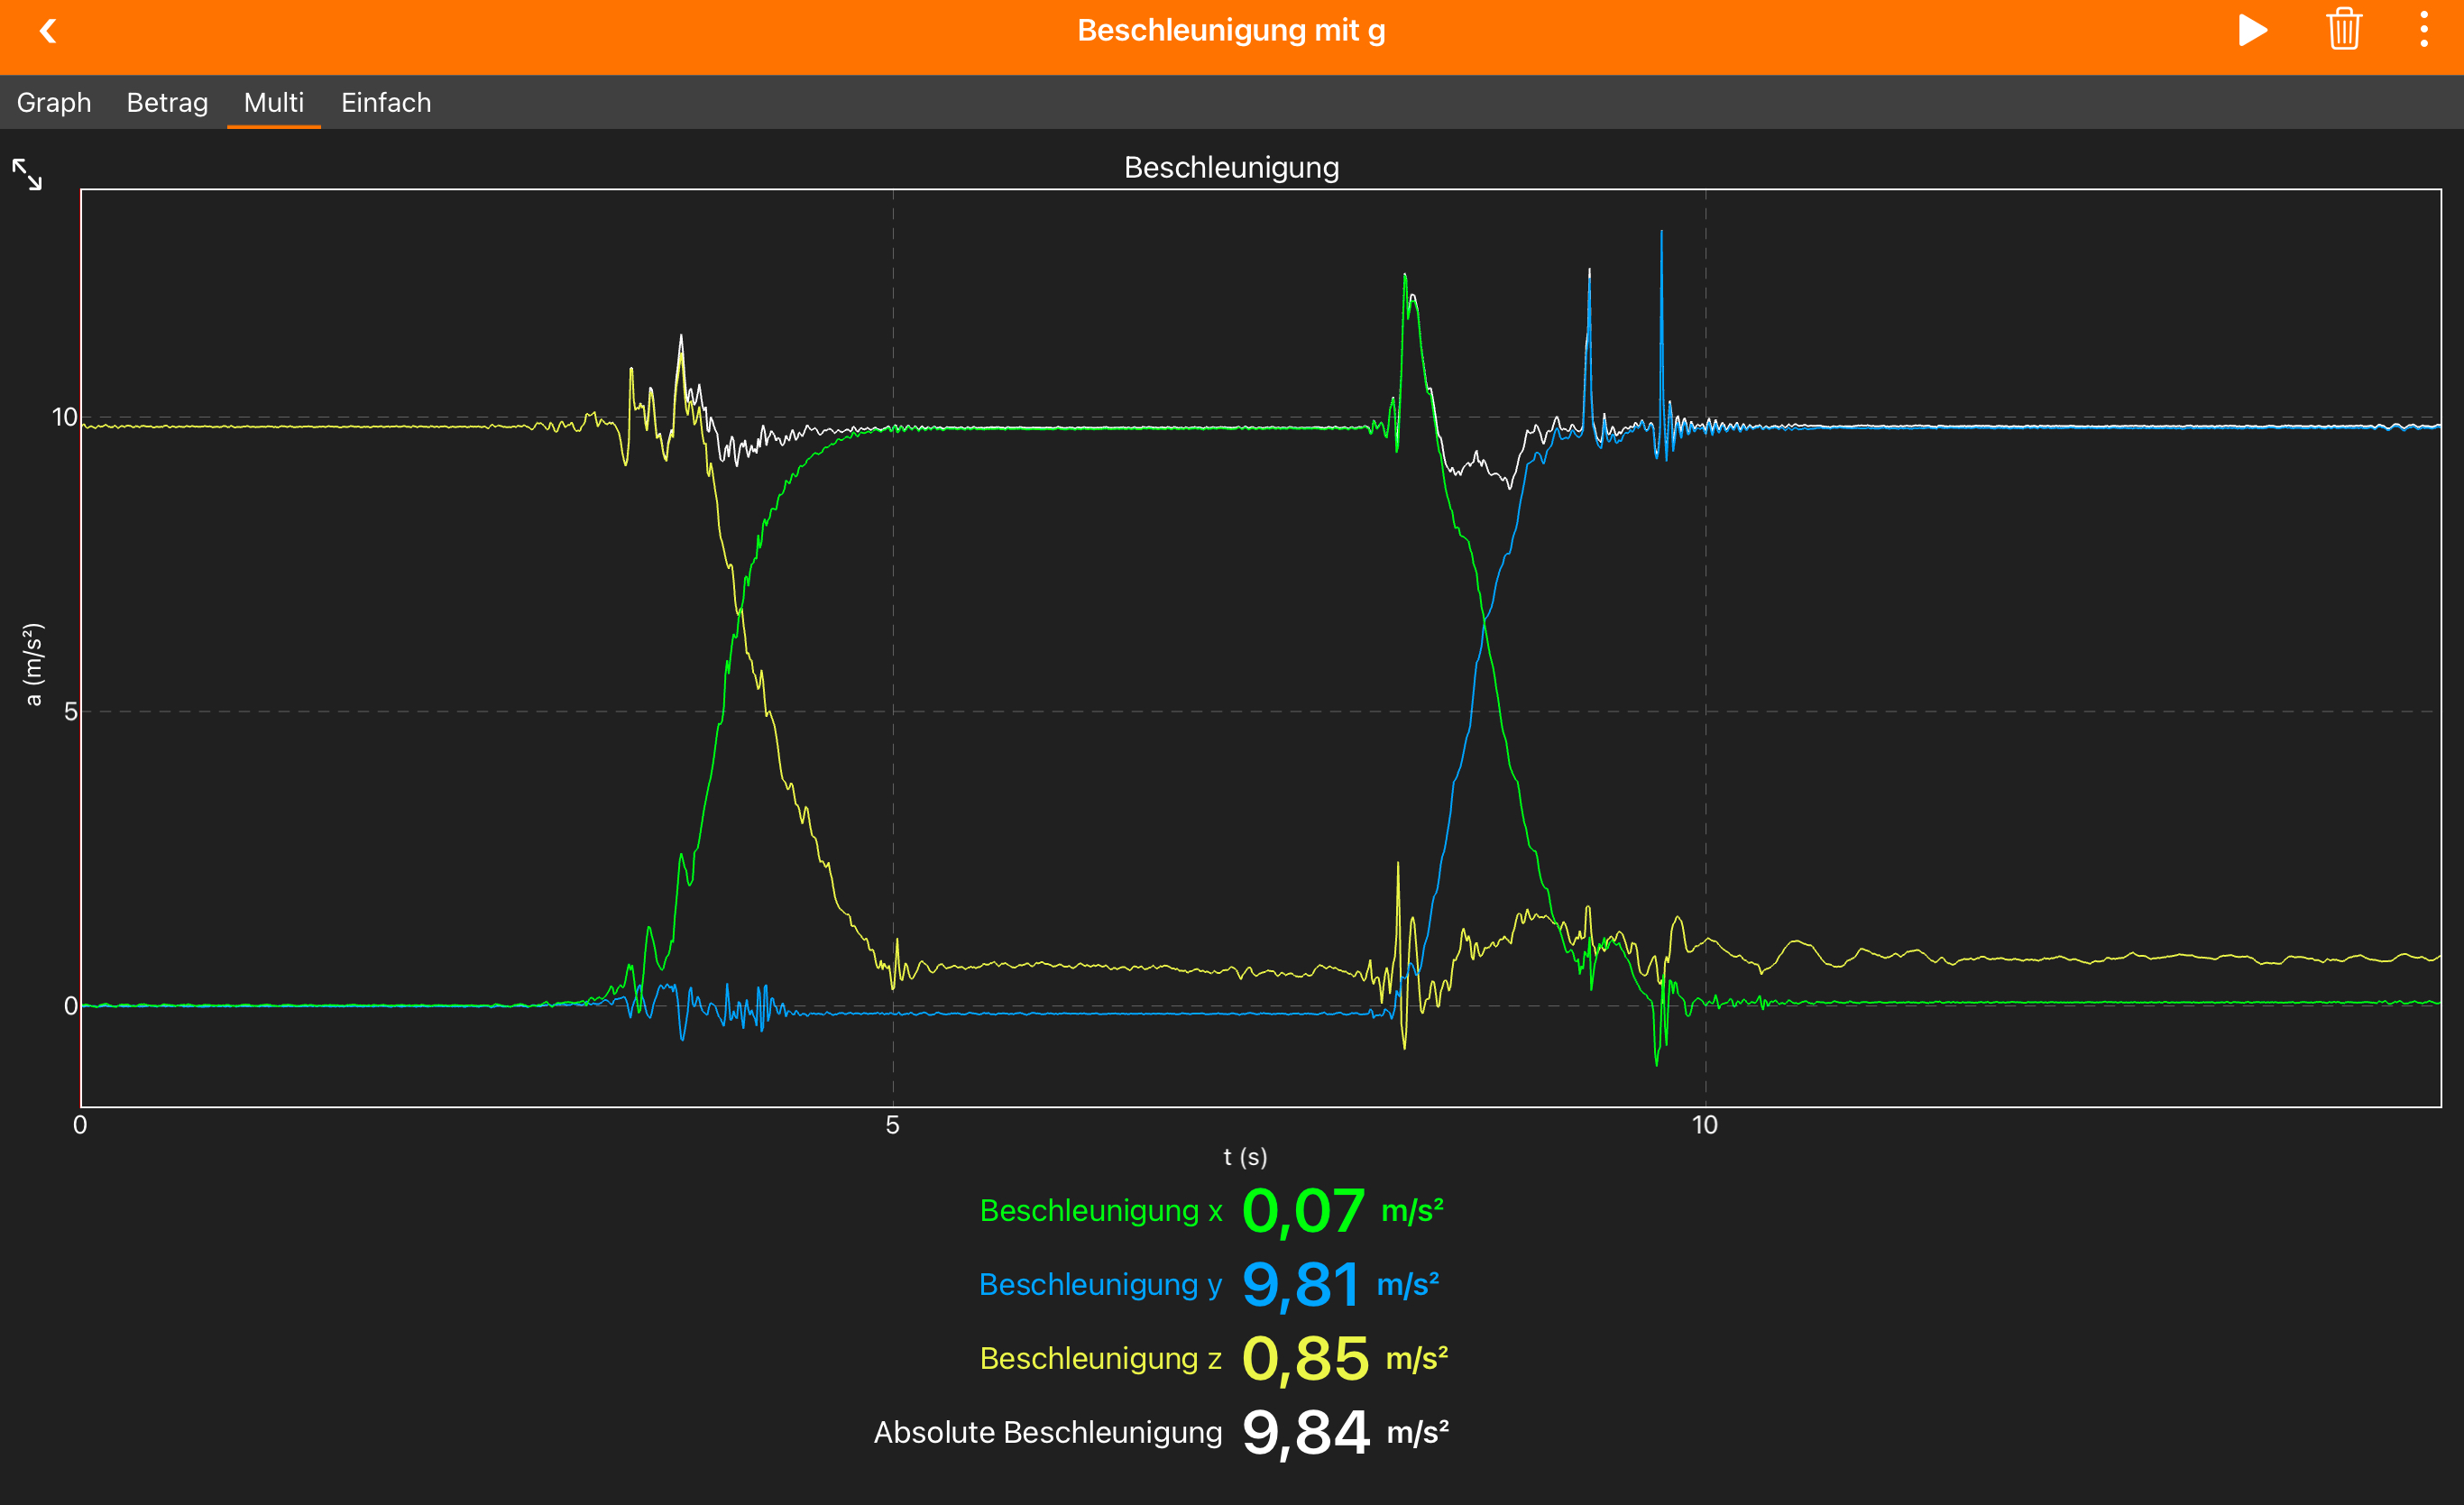
\includegraphics[width=0.75\linewidth]{images/Beschleunigung.jpeg}
\caption{Versuch Beschleunigungsdaten \cite{Phyphox}}
\label{fig:Versuch Beschleunigungsdaten}
\end{figure}
\begin{figure}[ht]\centering
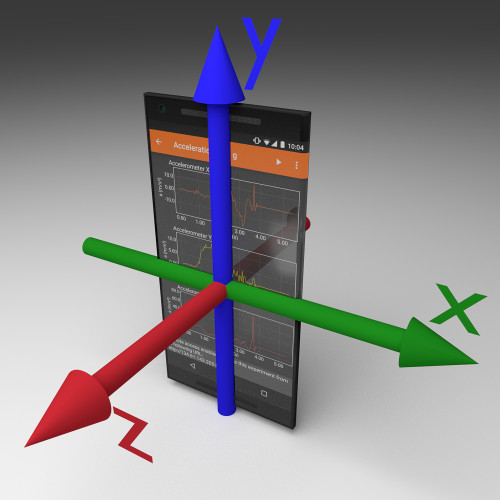
\includegraphics[width=0.35\linewidth]{images/Achsenzuordnung.jpeg}
\caption{Achsenzuordnung \cite{Phyphox}}
\label{fig:Achsenzuordnung}
\end{figure}
\\
\noindent Betrachtet man den Verlauf des Graphen, ist zunächst eine Beschleunigung von ca. 9,81 m/s² auf der Z-Achse zu erkennen, welches dem flachen liegen auf dem Tisch darstellt. Nach einigen Sekunden verlagert sich diese Annäherung an 9,81 m/s² auf die X-Achse, das Smartphone liegt nun auf der Längskante. Da das Smartphone nicht exakt gerade ausgerichtet ist, zeigt die Z-Achse weiterhin eine geringe Beschleunigung von etwa 0,8 m/s². Nach weiteren Sekunden wechselt die Annäherung an 9,81 m/s² auf die Y-Achse, das Smartphone steht jetzt aufrecht. Auch hier ist das Smartphone nicht vollkommen exakt ausgerichtet, sodass die Z-Achse erneut eine geringe Beschleunigung von etwa 0,8 m/s² anzeigt. Der beobachtete Verlauf der Kurven entspricht den Erwartungen
\\
\\
\noindent Für die Auswertung des Kniebeugewinkels wird jedoch nur die X-Achse und Y-Achse der beiden synchronisierten Smartphones benötigt. Die Z-Achse sind für diese Art der Analyse nicht relevant und werden daher vernachlässigt.